% Source: Unknown
% File: ".pdf"
% Access: Unknown

% comment out for student version
% \ifdefined\Student\relax\else\def\Teacher{}\fi

\documentclass[12pt]{article}

\title{Activity \#27: Recursion}
\author{Unknown}
\newcommand{\activityeditor}{Preston Carman}
\newcommand{\activitysource}{\url{}}
\date{Spring 2022}

\input{../../cspogil.sty}
\usepackage{tikz}

\begin{document}

  \begin{center}
    \maketitle
    \rolenames
  \end{center}
  
  \keyquestions{
    \item Model 1, Question \#2
    \item Model 2, Question \#7
    \item Model 3, Question \#17
  }

  \newpage
  \maketitle

  In this activity, you will work in teams of 3--4 students to learn new concepts.
  This activity will introduce you to recursion in C++.

  \guide{
    \item Identify the base case and recursive step of the
      factorial function
    \item Trace a recursive function by hand and and predict its
      final output
    \item Explain what happens in memory when a function
      calls itself
  }{
    \item Write a recursive function to compute the sum of
      the first $n$ numbers\\[-5pt]
  }{
    No additional notes.
  }

  \model{The Factorial Function}
  \begin{center}
    \renewcommand{\arraystretch}{1.2}
    \begin{tabular}{c|cccccc}
      $n$ & 0 & 1 & 2 & 3 & 4 & 5 \\
      \hline
      $n!$ & 1 & 1 & 2 & 6 & 24 & 120 \\
    \end{tabular}
  \end{center}
  
  {\it\large Refer to Model 1 above as your team develops consensus answers
    to the questions below.}

  \quest{15 min}

  \Q In mathematics, the {\it factorial} function for a natural
    number $n$ is denoted by $n!$.  It is the product of all positive
    integers less than or equal to $n$.  For example:
    \[
      5! = 5\times 4 \times 3 \times 2 \times 1 = 120
    \]
    Consider how to calculate $4!$.
    \begin{enumerate}
      \item Write out all of the numbers that need to be multiplied
        to get $4!$.
        \begin{answer}[0.5in]
          \[ 4! = 4\times 3\times 2\times 1 \]
        \end{answer}

      \item Rewrite the expression using $3!$ instead of $3\times
        2\times 1$.
        \begin{answer}[0.5in]
          \[ 4! = 4\times 3! \]            
        \end{answer}
    \end{enumerate}
    \par\vskip -40pt\null
    
  \Q Express the factorials as a product of a single
    natural number with a simpler factorial\key\\[-2mm].
    \begin{enumerate}
      \itemsep 10pt
      \begin{multicols}{2}
        \item $3! =$ \hspace{0.3in} \ans[2in]{$3 \times 2!$}
        \item $2! =$ \hspace{0.3in} \ans[2in]{$2 \times 1!$}
        \item $100! = $\hfill \ans[2in]{$100 \times 99!$}
        \item $n! = $\hfill \ans[2in]{$n\times (n-1)!$}
      \end{multicols}
    \end{enumerate}
    
  \item Now consider the very first natural number, 0.
    \begin{enumerate}
      \item Based on the model, what is the value of
        $0!$? \ans[1.5in]{1}\par\vskip 10pt

      \item Does it make sense to define $0!$ in terms of a simpler
        factorial?  Explain.        
        \begin{answer}[0.5in]
          No, we can't say that $0 \times -1! = 1$ because factorial
          is only defined for non-negative numbers.
        \end{answer}

      \newpage

      \item When we define the value of a function by
        referencing that same function for a simpler value, we will
        eventually reach a point where there are no simpler values
        and we have to just give a concrete value to the function.
        This is called a {\it base case}.  What is the base case for
        the factorial function?
        \begin{answer}[0.5in]
          The base case is $0! = 1$.
        \end{answer}
    \end{enumerate}

  \vskip -20pt
    
  \Q Suppose you already have a working implementation of the
    function declared below.
    \begin{center}
      \cpp{int factorial(int n);}
    \end{center}
    \begin{enumerate}
      \itemsep 10pt
      \item How could you compute $100!$ without calling
        \cpp{factorial(100)}?  Give a C++ command to do this.
        \begin{answer}[0.5in]
          \cpp{int result = 100 * factorial(99);}
        \end{answer}

      \item How could you compute $n!$ without calling
        \cpp{factorial(n)}?  Give a C++ command to do this.
        \begin{answer}[0.5in]
          \cpp{int result = n * factorial(n-1);}
        \end{answer}
    \end{enumerate}
  \newpage
  \model{A C++ Factorial Function}
    \begin{center}
      \begin{minipage}{5in}
        \begin{cpplst}
int factorial(int n) {
  cout << "n is " << n << endl;
  if (n == 0) {
    return 1;    // base case
  } else {
    cout << "need factorial of " << (n-1) << endl;
    int answer = factorial(n-1);
    cout << "factorial of " << (n-1) << " is " << answer << endl;
    return n * answer;
  }
}
        \end{cpplst}      
      \end{minipage}
    \end{center}

  {\it\large Refer to Model 2 above as your team develops consensus answers
    to the questions below.}

  \quest{15 min}
  
  \Q This model gives a definition of the
    \cpp{factorial} function.  Use it to answer the
    following questions.
    \begin{enumerate}
      \itemsep 10pt
      \item What specific function is called on line 10?
        \hfill\ans[2.5in]{The function \cpp{factorial} is called with the argument
        \cpp{n-1}.}

      \item Why is the \cpp{if} statement on line 6
        needed?
        \begin{answer}[0.5in]
          It defines the base case for the recursion.  Without it,
          the function would call itself indefinitely.
        \end{answer}       
    \end{enumerate}

  \vskip -30pt
    
  \Q A function that calls itself is called {\it recursive}.
    What two steps are required to define the recursive function
    \cpp}factorial}?
    \begin{answer}[0.75in]
    \end{answer}
    \par\vskip -30pt\null
    
  \Q Because recursive functions call themselves as a part of
    their execution, it takes some\key\\[-2.5mm] thought to understand 
    their execution.
    \begin{enumerate}
      \itemsep 10pt
      \item How many distinct function calls would be made to the
        \cpp{factorial} function to compute $2!$?
        Identify the function argument for each of those calls.
        \begin{answer}[0.5in]
          It would make three distinct calls:
          \cpp{factorial(2)}, \cpp{factorial(1)}, \cpp{factorial(0)}
        \end{answer}

      \item How many distinct function calls would be made to the 
        \cpp{factorial} function to compute $4!$?
        Identify the function argument for each of those calls.
        \begin{answer}[0.5in]
          It would make five distinct calls:
            \cpp{factorial(4)}, \cpp{factorial(3)}, \cpp{factorial(2)}
            \cpp{factorial(1)}, \cpp{factorial(0)}
        \end{answer}
    \end{enumerate}

  \vskip -20pt
    
  \Q The file {\tt activity27a.cpp.cpp} contains the function from    
    this model along with a test function call to compute $5!$.  Run
    this program and then identify the function call which produces
    each line of output below.  Several have been done for you.    
    \begin{enumerate}
      \itemsep 10pt
      \begin{multicols}{2}
        \item {\tt n is 5} \hspace{1.3in}\underline{\tt{factorial(5)}}
        \item {\tt need factorial of 4} \hspace{0.2in}\ans[1in]{\tt{factorial(5)}}
        \item {\tt n is 4} \hspace{1.3in}\ans[1in]{\tt{factorial(4)}}
        \item {\tt need factorial of 3} \hspace{0.2in}\ans[1in]{\tt{factorial(4)}}
        \item {\tt n is 3} \hspace{1.3in}\ans[1in]{\tt{factorial(3)}}
        \item {\tt need factorial of 2} \hspace{0.2in}\ans[1in]{\tt{factorial(3)}}
        \item {\tt n is 2} \hspace{1.3in}\ans[1in]{\tt{factorial(2)}}
        \item {\tt need factorial of 1} \hspace{0.2in}\underline{\tt{factorial(2)}}
        \item {\tt n is 1} \hfill\ans[1in]{\tt{factorial(1)}}
        \item {\tt need factorial of 0} \hfill\ans[1in]{\tt{factorial(1)}}
        \item {\tt n is 0} \hfill\ans[1in]{\tt{factorial(0)}}
        \item {\tt factorial of 0 is 1} \hfill\underline{\tt\hspace{5pt}factorial(1)\hspace{5pt}}
        \item {\tt factorial of 1 is 1} \hfill\ans[1in]{\tt{factorial(2)}}
        \item {\tt factorial of 2 is 2} \hfill\ans[1in]{\tt{factorial(3)}}
        \item {\tt factorial of 3 is 6} \hfill\ans[1in]{\tt{factorial(4)}}
        \item {\tt factorial of 4 is 24} \hfill\ans[1in]{\tt{factorial(5)}}
      \end{multicols}
    \end{enumerate}
    
  \Q What happens if you try to calculate the factorial of a
    negative number?  Explain why this happens.
    \begin{answer}[0.5in]
      It results in a stack overflow error because the base case
      is never reached and the function keeps calling itself
      indefinitely.
    \end{answer}
    
  \Q How could you prevent this behavior?
    \begin{answer}[0.5in]
      You could add an additional \cpp{if} statement to check if
      the argument is negative and handle that case appropriately,
      such as returning an error value or printing an error message.
    \end{answer}

  \Q What is the largest factorial you can compute in C++ without
    changing the types of the variables in this function?  Play with
    the code in {\tt activity08.cpp} to find out.
    \begin{answer}[0.5in]
      The largest factorial that can be computed without changing
      the variable types is 12! because 13! exceeds the maximum
      value for an \cpp{int}.
    \end{answer}

  \newpage
  \model{Summations}
  \begin{center}
    \[
      \sum_{i=1}^{100} i = 1 + 2 + 3 + \cdots + 100 = 5050
    \]
  \end{center}
  
  {\it\large Refer to Model 3 above as your group develops consensus answers
    to the questions below.}

  \quest{20 min}
    
  \Q In mathematics, {\it summation} (represented by the Greek
    letter ``sigma'', $\Sigma$) is the addition of a sequence of
    numbers resulting in a single sum or total. For example, 
    \[
      \sum_{i=1}^{i=3} i = 1 + 2 + 3 = 6
    \]
    \vskip -10pt\null
    Consider how to calculate $\displaystyle \sum_{i=1}^{5} i$.
    \begin{enumerate}
      \itemsep 10pt
      \item Write out all the numbers that need to be added.
        \begin{answer}[0.5in]
          \[ 1 + 2 + 3 + 4 + 5 \]
        \end{answer}

      \item Show how this sum can be calculated in terms of a smaller
        summation.
        \begin{answer}[0.5in]
          \[ \sum_{i=1}^{5} i = 5 + \sum_{i=1}^{4} i \]
        \end{answer}
    \end{enumerate}
      
  \Q Express the summations as a sum of a single
    natural number and a shorter summation.
    \begin{enumerate}
      \itemsep 10pt
      \begin{multicols}{2}
        \item $\displaystyle \sum_{i=1}^{100} i = $ \hspace{0.2in} \ans[2in]{$100 +
          \sum_{i=1}^{99} i$}
        \item $\displaystyle \sum_{i=1}^n i = $ \hfill \ans[2in]{$n +
          \sum_{i=1}^{n - 1} i$}
      \end{multicols}
      \item The base case for this summation is: \hfill\ans[2in]{$\sum_{i=1}^{1} i = 1$}
    \end{enumerate}

  \Q Write a C++ function {\tt summation} that takes a single
    parameter {\tt n} and returns the sum $1 + 2 + \cdots + n$.  It
    should only have an \cpp{if} statement and two 
    \cpp{return} statements.
    \begin{answer}[1in]
      Answers will vary
    \end{answer}

  \newpage
    
  \Q Below is a different recursive implementation of the
    {\tt factorial} function seen in model 2.
    \par\vskip -20pt\null
    \begin{center}
      \begin{tabular}{p{2.7in}p{3.7in}}
        \begin{minipage}{2.7in}
          \begin{cpplst}
int factorial(int n) {
  if (n == 0) {
    return 1; // base case
  }
  int recurse = factorial(n-1);
  int result = n * recurse;
  return result;
}
          \end{cpplst}
        \end{minipage}
        &
        \begin{minipage}{3.7in}
          \begin{enumerate}
            \item How are temporary variables used in this function?
              \begin{answer}[0.5in]
                They store the results of the recursive call and
                the final result before returning it.
              \end{answer}

            \item What would you change to change this to a {\tt
              summation} function?
              \begin{answer}[0.5in]
                Change the multiplication to addition in the line
                calculating {\tt result}.
              \end{answer}              
          \end{enumerate}
        \end{minipage}
      \end{tabular}
    \end{center}

    \vskip -30pt
        
  \Q Below is a {\it stack diagram} of a call to this implementation
    of \cpp{factorial(3)} from the\key\\[-2.5mm] {\tt main} program.
    Sketch a similar diagram for a call to \cpp{summation(3)}.
    \begin{center}
      \begin{tabular}{p{3in}p{3in}}
        \begin{minipage}{3in}
          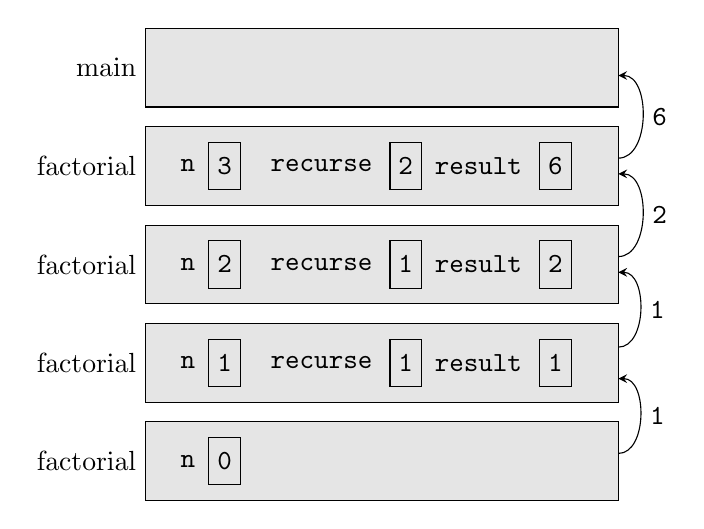
\begin{tikzpicture}
          
            \draw[fill=gray!20] (0,5) rectangle (6,6);
            \node[left] at (0,5.5) {main};
            \draw[fill=gray!20] (0,3.75) rectangle (6,4.75);
            \node[left] at (0,4.25) {factorial};
            \node[left] at (0.75,4.25) {\tt n};
            \draw (0.8,3.95) rectangle (1.2,4.55) node[pos=.5] {\tt 3};
            \node[left] at (3,4.25) {\tt recurse};
            \draw (3.1,3.95) rectangle (3.5,4.55) node[pos=.5] {\tt 2};
            \node[left] at (4.9,4.25) {\tt result};
            \draw (5,3.95) rectangle (5.4,4.55) node[pos=.5] {\tt 6};
          
            \draw[fill=gray!20] (0,2.5) rectangle (6,3.5);
            \node[left] at (0,3) {factorial};
            \node[left] at (0.75,3) {\tt n};
            \draw (0.8,2.7) rectangle (1.2,3.3) node[pos=.5] {\tt 2};
            \node[left] at (3,3) {\tt recurse};
            \draw (3.1,2.7) rectangle (3.5,3.3) node[pos=.5] {\tt 1};
            \node[left] at (4.9,3) {\tt result};
            \draw (5,2.7) rectangle (5.4,3.3) node[pos=.5] {\tt 2};
          
            \draw[fill=gray!20] (0,1.25) rectangle (6,2.25);
            \node[left] at (0,1.75) {factorial};
            \node[left] at (0.75,1.75) {\tt n};
            \draw (0.8,1.45) rectangle (1.2,2.05) node[pos=.5] {\tt 1};
            \node[left] at (3,1.75) {\tt recurse};
            \draw (3.1,1.45) rectangle (3.5,2.05) node[pos=.5] {\tt 1};
            \node[left] at (4.9,1.75) {\tt result};
            \draw (5,1.45) rectangle (5.4,2.05) node[pos=.5] {\tt 1};
          
            \draw[fill=gray!20] (0,0) rectangle (6,1);
            \node[left] at (0,0.5) {factorial};
            \node[left] at (0.75,0.5) {\tt n};
            \draw (0.8,0.2) rectangle (1.2,0.8) node[pos=.5] {\tt 0};
            
            \draw[-stealth] (6,0.6) to [out=0,in=0] node[right] {\tt 1} (6,1.55);
            \draw[-stealth] (6,1.95) to [out=0,in=0] node[right] {\tt 1} (6,2.9);
            \draw[-stealth] (6,3.1) to [out=0,in=0] node[right] {\tt 2} (6,4.15);
            \draw[-stealth] (6,4.35) to [out=0,in=0] node[right] {\tt 6} (6,5.4);
            
          \end{tikzpicture}
        \end{minipage}
        &
        \begin{minipage}{3in}
        \end{minipage}
      \end{tabular}
    \end{center}
  \begin{enumerate}
    \item Why are there no values for {\tt recurse} and {\tt result}
      in the stack diagram for the last call to {\tt factorial} (when
      \cpp{n == 0}?      
      \begin{answer}[0.5in]
        Because in that case, the function hits the base case and
        returns 1 immediately without calculating those variables.
      \end{answer}
      
    \item Looking at the stack diagram, how is it possible that the
      parameter {\tt n} can have multiple values in memory at the same
      time?
      \begin{answer}[0.5in]
        Each function call has its own separate stack frame in memory,
        so each call to {\tt factorial} has its own copy of the
        parameter {\tt n}.
      \end{answer}
  \end{enumerate}


\end{document}